\section{Messstruktur für Analog-Digital-Wandler}
	
Nach der Einführung in die grundlegenden Funktionen von LabVIEW wurde die Programmierumgebung genutzt, um einfache Messstrukturen zu erstellen.
Dazu wurden ein analoger Funktionsgenerator und ein Analog-Digital-Wandler (ADC) zur Verfügung gestellt.
Über den Wandler ließ sich der Funktionsgenerator an den Computer anschließen.
Da der verwendete Wandler von National Instruments (ebenfalls Urheber von LabVIEW) hergestellt wurde, konnte dieser unter LabVIEW direkt erkannt und ohne komplizierten Einrichtungsprozess verwendet werden.

\subsection{DAQ-Assistant}

Mit einem vorprogrammierten Express-VI, dem DAQ-Assistant (siehe Abb. \ref{fig:daq}), konnten die mit dem Funktionsgenerator erzeugten Signale gemessen werden.

\begin{figure}[ht]
	\centering
	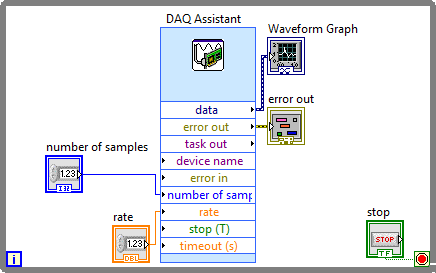
\includegraphics[width=0.8\textwidth]{pic/daq.png}
	\caption{Diese Abbildung stellt das Express-VI "DAQ-Assistant" dar. Darauf sind die verschiedenen Ein- und Ausgänge zu sehen.}
	\label{fig:daq}	
\end{figure}

Lediglich die Anzahl der Datenpunkte und die Messrate mussten dem DAQ-Assistant geliefert werden damit ein Waveform-Graph aus dem Array, welches der "data"-Ausgang ausgab, das Bild in Abb. \ref{fig:daq_sig} erzeugt werden konnte. Das aufgezeichnete Signal stimmte mit dem überein, was an dem Funktionsgenerator eingestellt wurde.

\begin{figure}[ht]
	\centering
	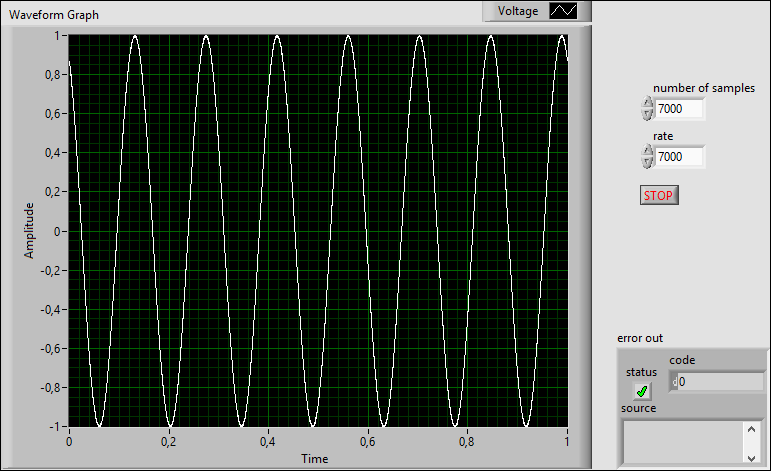
\includegraphics[width=\textwidth]{pic/daq_sig.png}
	\caption{Diese Abbildung stellt das Frontpanel eines VIs mit dem DAQ-Assistant und Controls für Messrate und Anzahl der Datenpunkte dar.}
	\label{fig:daq_sig}	
\end{figure}



\subsection{Programmieren einer eigenen Messstruktur}

Da lediglich eine Anzeige des gemessenen Signals oft nicht reicht, musste eine Messstruktur programmiert werden, die den Umfang des DAQ-Assistants übersteigt und weiter manuell angepasst werden kann.
	
\

Aufgrund von Problemen bei Wartungsarbeiten ließen sich die Computer jedoch gegen Mittag nicht mehr bedienen, weswegen das Fertigstellen des Programms auf den Folgetag verschoben wurde. 
Zur Vorbereitung für das Weiterarbeiten wurden thematisch noch die Fouriertransformation zur Spektralanalyse, so wie das Abtasttheorem für eine richtige Messung angesprochen.
	
\

